\section{Methods}
In the literature there are multiple approaches for verification and testing of implemented swarm behaviours. There are several works which document algorithms for those behaviours with the related experiments and results \cite{Formal_Verification_of_Probabilistic_Swarm_Behaviours},\cite{Towards_Temporal_Verification_of_Emergent_Behaviours_in_Swarm_Robotic_Systems}, \cite{Property-driven_design_for_swarm_robotics}. In some cases there is an automaton corresponding to the textual description of behaviour or pseudocode \cite{Formal_Verification_of_Probabilistic_Swarm_Behaviours}. At times, used logic and tools are mentioned \cite{Property-driven_design_for_swarm_robotics}. However we are not be able to reproduce the experiments because none of the works explained in detail how the chosen swarm behaviour was modelled. That is why this section will focus on explaining how algorithm's pseudocode and general assumptions are transformed into a functioning model. The selected algorithm to demonstrate the process of modelling is Alpha algorithm. It was chosen because there were many experiments that addressed Alpha algorithm but omitted the details of what was actually being tested or verified \cite{Towards_Temporal_Verification_of_Emergent_Behaviours_in_Swarm_Robotic_Systems}, \cite{On_Formal_Specification_of_Emergent_Behaviours_in_Swarm_Robotic_Systems}.

\subsection{Alpha algorithm}
Alpha algorithm was introduced by Julien Nembrini in \cite{Minimalist_Coherent_Swarming_of_Wireless_Networked_Autonomous_Mobile_Robots}. It was inspired by Kasper Støy's work \cite{Using_Situated_Communication_in_Distributed_Autonomous_Mobile_Robotics}. Støy proposed and implemented a simple control system for aggregating robots. Instead of relying on environment and localisation information, it uses physical properties of the signal used for communication. Robot behaviour is solely determined by the change in the number of robots that are in the range of its signal.

Alpha algorithm is an approach to an aggregation task within the category of spatial organisation. It is based on the assumption that robots send and receive signals through omnidirectional channels like radio or infrared. Single robots make decisions about their movement only based on the number of connections to other robots. The inter-connectivity of the swarm is controlled by the alpha parameter which is a threshold on the desired number of connections for a single robot. Pseudocode defining the Alpha algorithm can be found in Figure \ref{fig:pseudocode}. Variable \textbf{i} in the pseudocode is a loop iterator and \textbf{cadence} is a parameter that controls how often a robot will send its ID and check the number of neighbours.

In order to explain the Alpha algorithm in a greater detail we will divide the most important aspects of the robot behaviour into subsections. First three subsections, namely, Movement, Connection, Initialisation and clocks, will explain the algorithm's general assumptions and design choices. The fourth and last subsection - Automaton, will transform the pseudocode for the Alpha algorithm into timed automaton while incorporating design choices introduced in previous subsections.

\begin{figure}[H]
\caption{Pseudocode for Alpha algorithm from \cite{Minimalist_Coherent_Swarming_of_Wireless_Networked_Autonomous_Mobile_Robots}}
\begin{lstlisting}
Create a list of neighbours for robot, Nlist
k = number of neighours in Nlist
i = 0

loop forever {
	i = i modulo cadence

	if (i = 0){
		Send ID message

		Save copy of k in LastK
		k = number of neighbours in Nlist

		if ((k < lastK) and (k < alpha)){
			turn robot through 180 degrees
		}
		else if (k > LastK) {
			make random turn
		}
	}

	Steer the robot according to state
	Listen for calls from robots in range
	Grow Nlist with neighbours IDs

	i++
}
\end{lstlisting}
\label{fig:pseudocode}
\end{figure}


\subsection{Movement}
There would be no need for Alpha algorithm without the robot movement so it is important to define how it is modelled. Robot always moves in one of four directions: up, right, down or left. Initial direction is chosen at random and mapped to vertical and horizontal components. Direction will not change unless the robot performs random turn or 180 degree turn. Random turn chooses new direction in the same way that initial direction is determined. This means that random turn may result in maintaining the current direction of the robot with approximately 25\% chance. 

Robot movement is achieved by incrementing the robot's coordinates with vertical and horizontal direction components. Direction component values are  $\in \{-1, 0, 1\}$, but either vertical or horizontal direction component has to be equal to zero. This means that robot will move in one of four possible directions with a step size equal to one. Every time the robot moves, it will update its coordinates in the globally available data structure. Environment in which robot exists is an unbounded grid that can be continuously traversed in four directions.

Robots are not aware of other robots positions. This means that they can occupy exactly the same point of the grid. Additionally, there is no collision avoidance mechanism that would prevent them from crashing into each other while moving. This simplification could be eliminated but at the cost of implementation being further apart from the original idea of what is an Alpha algorithm. We would have to make arbitrary decisions about robot behaviour in the case of collision or inability to move to the occupied point on the grid.

\subsection{Connection}
Number of robot connections is the main parameter determining the robot behaviour. Therefore it is important to accurately model what it means for robots to be connected. One of the assumptions in Julien Nembrini's \cite{Minimalist_Coherent_Swarming_of_Wireless_Networked_Autonomous_Mobile_Robots} is that physical signal is omnidirectional. However, robot movement is modelled to be two dimensional. Consequently we will assume that two robots are connected if their distance is smaller than radius of physical signal that we mimic. Length of the radius will determine how far apart the robots can move before losing connection.

To model the physical signal we need information about robot coordinates, mutual distances, previous and current number of neighbours. This allows for evaluating whether robots are in the signal distance and therefore connected or not. Every time robot moves it will update its own coordinates, previous number of neighbours for itself, current number of neighbours for all robots and mutual distances for all robots. It may seem like the robot is using more information than it is assumed in the Alpha algorithm. Information that it passes is used to mimic the physical signal of the real robot. Although, it updates its coordinates, robot is not aware of the position of its neighbours. Its movement is derived solely from information about previous and current number of neighbours. 

The desired number of connections is set by the alpha parameter. If the number of connections falls below alpha, robot will react and turn 180 degrees in order to try to reconnect with other robots. Alpha parameter influences connectivity of the swarm. If the parameter is set to higher values the robots will try to maintain more connections and the resulting swarm will be more compact. If the parameter is set to lower values, robots will be able to move further apart as they will need to maintain less connections. What is low and high value for alpha parameter is subjective to the size of the swarm.

\subsection{Initialisation and clocks}
This subsection explains the initial state of the robot and the influence that the time has on its behaviour. Every robot gets initialised with the same set of parameters apart from its ID. In the beginning all robots are placed at exactly the same point. They have no direction until transitioning to the next state - RANDOM STATE, and will not move forward until transitioning further. In the INITIAL state robots cannot access information about number of current neighbours and number of last neighbours. The INITIAL state becomes unreachable after the robot transitions from it.

Pseudocode variables \textbf{i} and \textbf{cadence} model the frequency of robot actions. Specifically \textbf{cadence}, it controls how often a robot sends a signal and checks if it should change direction. While we are able to model such frequency without a timed automaton we would not be able to model a real-time system like robot swarm. The timing aspect allows us to model a system with time dependent behaviours and to verify a time dependent properties. We can observe a system behaviour throughout time and evaluate the stability of the implemented algorithm. That is why each robot has its own clock that controls how long it can remain in the current state before being forced to transition. After each transition to the next state the robot will reset its own clock. Maximum time for the robot to remain in state can influence the behaviour of the whole system. If we decrease the maximum time of inactivity, we will obtain a system that is on average more reactive and even. With increasing the maximum time of inactivity we increase the chances of robots operating in different pace. As we are modelling swarm we should aim for uniform operation and therefore lower maximum times for inactivity.

\subsection{Automaton}
In order to implement the Alpha algorithm presented in \cite{Minimalist_Coherent_Swarming_of_Wireless_Networked_Autonomous_Mobile_Robots}, we utilised the pseudocode from Figure \ref{fig:pseudocode}, with design choices described in the previous subsections. The implementation is a timed automaton - Figure \ref{fig:automaton}.

We will describe how pseudocode was mapped into the timed automaton. Pseudocode starts with creating and initialising variables that are needed for algorithm execution. This part is not explicitly visible in the automaton but achieved during initialisation of the model.\\\\
Pseudocode variables that represent the state:\\
- \textbf{Nlist}, a list of neighbours for a robot;\\
- \textbf{ID}, a unique robot identifier;\\
- \textbf{k}, a number of neighbours in Nlist;\\
- \textbf{lastK}, a previous number of neighbours in Nlist;\\
- \textbf{alpha}, a threshold on the number of connections;\\

 The state of the algorithm before entering the infinite loop is represented by the INITIAL state. Transitioning from the INITIAL state is equivalent to entering the infinite loop defined in the pseudocode. The entry point for the loop is a RANDOM TURN state where the robot obtains its initial random direction. Infinite loop defines that robot will send its ID and make a decision about turning only every 'cadence' loop iterations. To mimic this behaviour cadence was implemented as the maximum time of inactivity $T$. In the pseudocode  decision about turning is realised with 'if' and 'if else' statements. Statements and their corresponding conditions were transformed to IF and IF ELSE states with conditions guarding subsequent transitions. Guarded transitions utilise original conditions and their negations. In this way we can guarantee that there is always only one transition possible at any point. Variables used in the conditions correspond to the current number of neighbours, previous number of neighbours and desired number of neighbours. Those variables control the behaviour of a single robot alongside the maximum time of inactivity $T$ which acts as a cadence parameter of the loop. Single robot is represented by the timed automaton presented in Figure \ref{fig:automaton}. Composition of such timed automata results in a robot swarm implementation of the Alpha algorithm. The movement and interactions of robots cause them to update their variables. Those variables are then used to determine the logical value of conditions guarding the state transitions. Finally, the available transitions are taken, influencing the robots behaviours. This process restarts and lasts indefinitely as the system composed of timed automata has no final state.\\

\noindent State descriptions:\\
- INITIAL, where the robot is not moving and has no direction;\\
- RANDOM TURN, where the robot randomly chooses one of four directions;\\
- U-TURN, where the robot changes direction by 180 degrees;\\
- FORWARD, where the robot moves forward in the set direction;\\
- IF, where the robot checks if it is disconnected from neighbours;\\
- ELSE IF, where the robot checks if it is connected to more than desired number of neighbours;\\\\
States are not enough to define the behaviour if the robot is not forced to transition. Each robot has its own clock that controls how much time it can remain in a given state. Time - $t$ a robot can remain in states FORWARD and INITIAL is limited by the maximum time $T$.
Robot has to transition before time $t$ is equal to $T$. After leaving mentioned states, the robot resets its clock. In remaining states the time doesn't pass and therefore time $t$ is not incremented. However other transitions are guarder by associated conditions. Transition from one state into another can only happen if the corresponding condition is satisfied. If there is no condition over the edge, transition can always be taken.\\\\ Conditions controlling the robot are associated with the following variables:\\
$n$ - current number of neighbours;\\
$l$ - previous number of neighbours;\\
$\alpha$ - Alpha parameter, desired number of neighbours;\\
\begin{figure}[H]
\caption{Timed automaton for the Alpha algorithm}
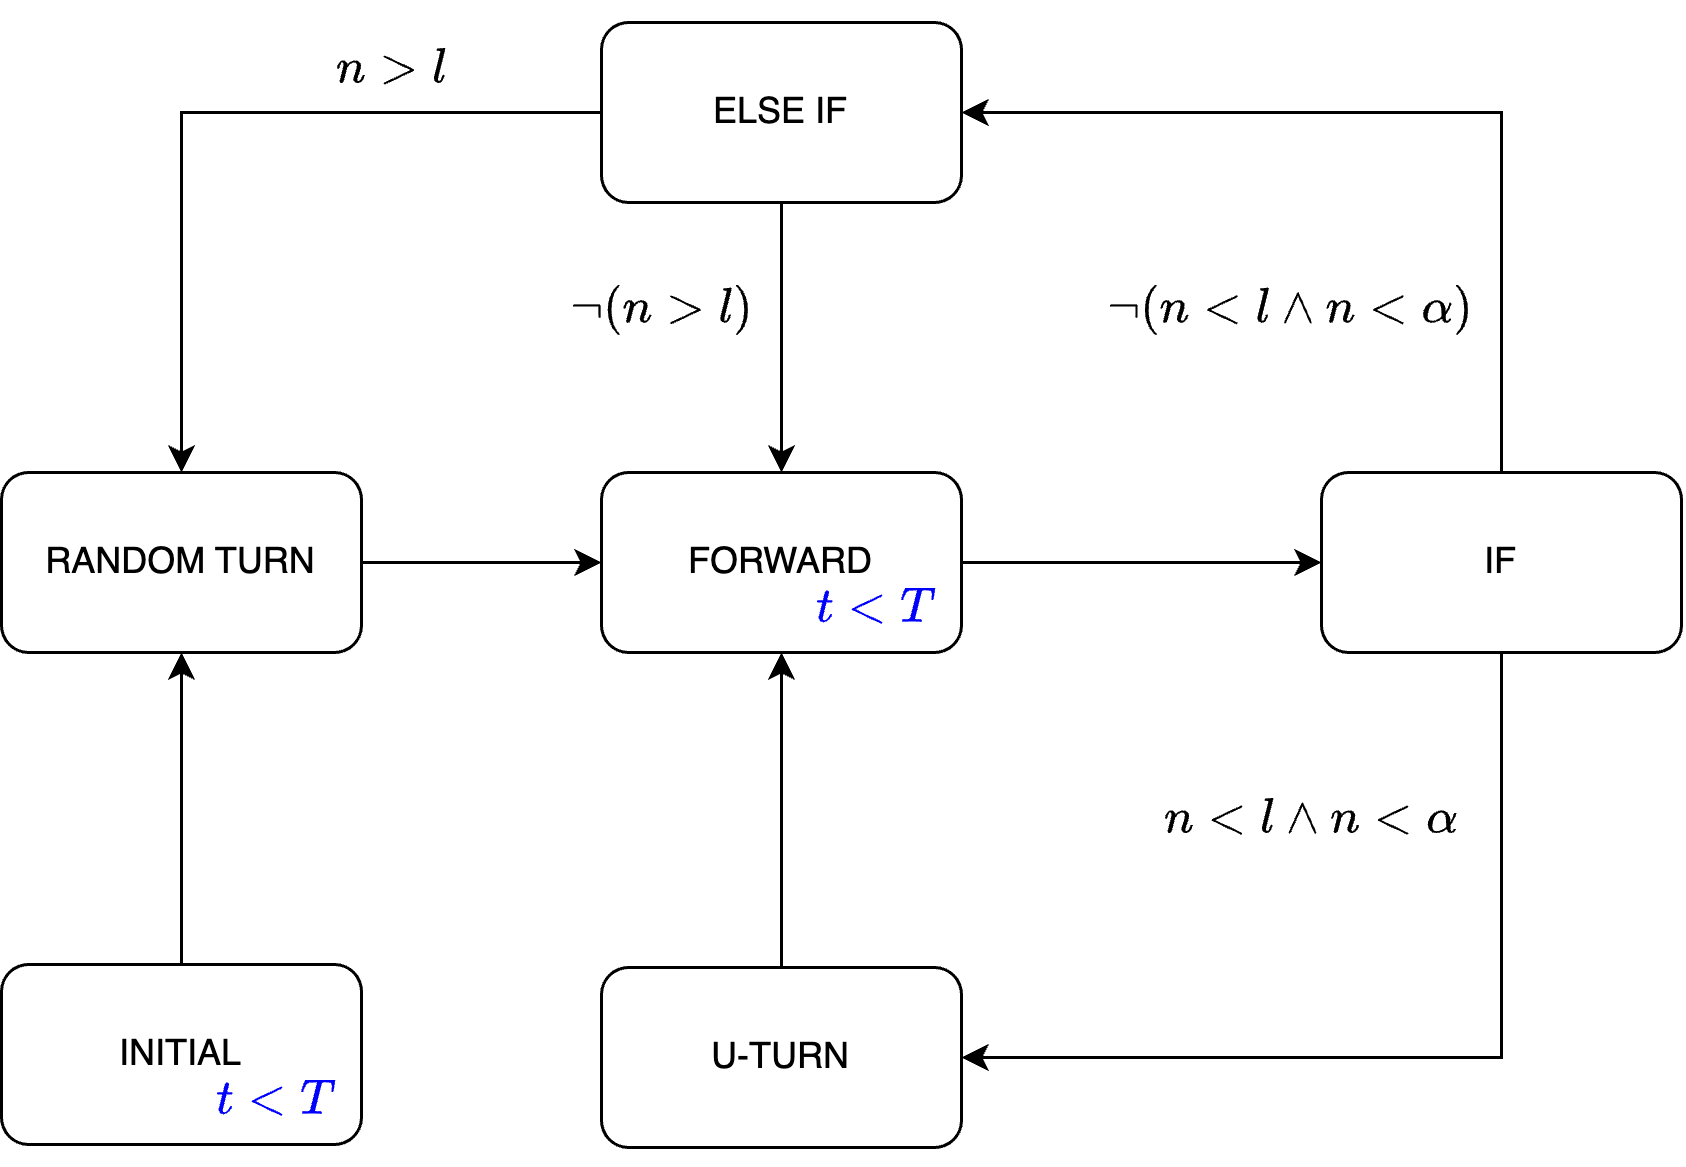
\includegraphics[scale=0.9]{images/automaton.png}
\label{fig:automaton}
\end{figure}